\section{Synchrotron X-ray Sources}

\begin{slide}{Generating X-rays}
  
  \begin{columns}
    \begin{column}{60mm}
      
      
      Light is generated by accelerating charge.
      \vmm
      
      \hspace{12mm} 
\includegraphics[width=15mm]{figs/Images/radio_tower}
      
      Accelerating low energy electrons gives low energy light:
      
      \vmm

      An AC current in a radio tower produces radio waves:
      $\rm \lambda \sim 1 m$,  $E \sim \rm 1 {\mu}eV$.

      \vmm\vmm\vmm

      X-rays have
      $\rm \lambda \sim 10^{-10} m$,  $E \sim \rm 10 keV$.
      
      \end{column}
      \begin{column}{75mm}

        {\onslide+<2> {

            \hspace{5mm} 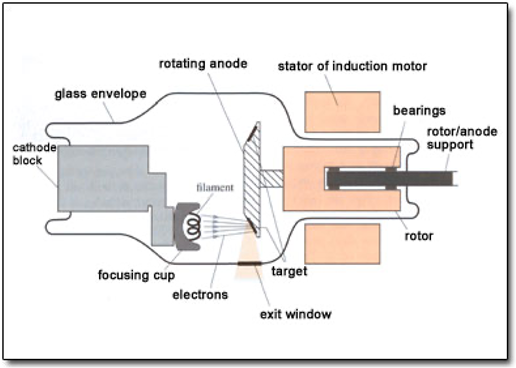
\includegraphics[width=60mm]{figs/Images/XrayTube}        


          \vmm\vmm
          
          An X-ray tube (lab, dentist office) slams electrons into a metal
          target.

          \vmm\vmm
          
          X-rays are produced from both X-ray fluorescence of the metal
          (discrete energies), and from the deceleration of the electrons.
          
          
          \vspace{2mm}
        }
      }
      \end{column}
    \end{columns}          
    
    \vmm \vfill
  \end{slide}
 

\begin{slide}{Synchrotron: a modern X-ray source}

  Accelerating high-energy electrons by turning them in a magnetic field
  gives very high fluxes.

    \begin{columns}
      \begin{column}{70mm}

        {\onslide+<2-> {
            \begin{enumerate}

           \item start with very high energy
             electrons  ($\sim 7\rm\, GeV$ at APS).  That's 14,000x the
             rest mass of an electron -- highly relativistic.
             
           \item keep the electrons going around
             a large ring for many hours.
             
           \item X-rays come off at tangents at every
             {\RedEmph{bending magnet}} - each gives a ``beamline''.

             {\onslide+<3-> {
               \item insert alternating magnet poles ({\RedEmph{wigglers}} or
             {\RedEmph{undulators}}) in straight sections between the
             bending magnets, bends the electron beam many times, giving
             beamlines with more and brighter X-rays!
             }}
           \end{enumerate}
         }}
           \vmm
           {\onslide+<3-> {           
           \hspace{9mm}
           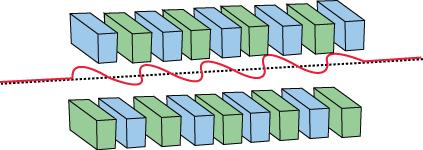
\includegraphics[width=42mm]{figs/Images/insertiondevice}

           \vspace{3mm}
           
           \vfill
           
           }}
         \end{column}
         \begin{column}{60mm}
           \vmm
           
           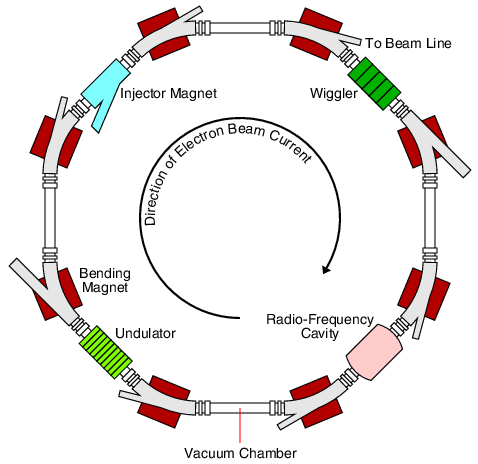
\includegraphics[width=50mm]{figs/Images/synchrotron_ring}

        {\onslide+<3-> {
           \vmm\vmm
           A {\RedEmph{synchrotron}} or {\RedEmph{storage ring}}, with many
           beamlines running simultaneously.
           
           \vmm US DOE runs 4 synchrotrons as User Facilities, with many
           more around the world.
           }}
         \end{column}
       \end{columns}


    \vmm \vfill


\end{slide}


\begin{slide}{Synchrotron: Brilliance and Spectral Ranges}

\vmm
\begin{columns}[T]
  \begin{column}{57mm}
    \onslide+<1-> {
      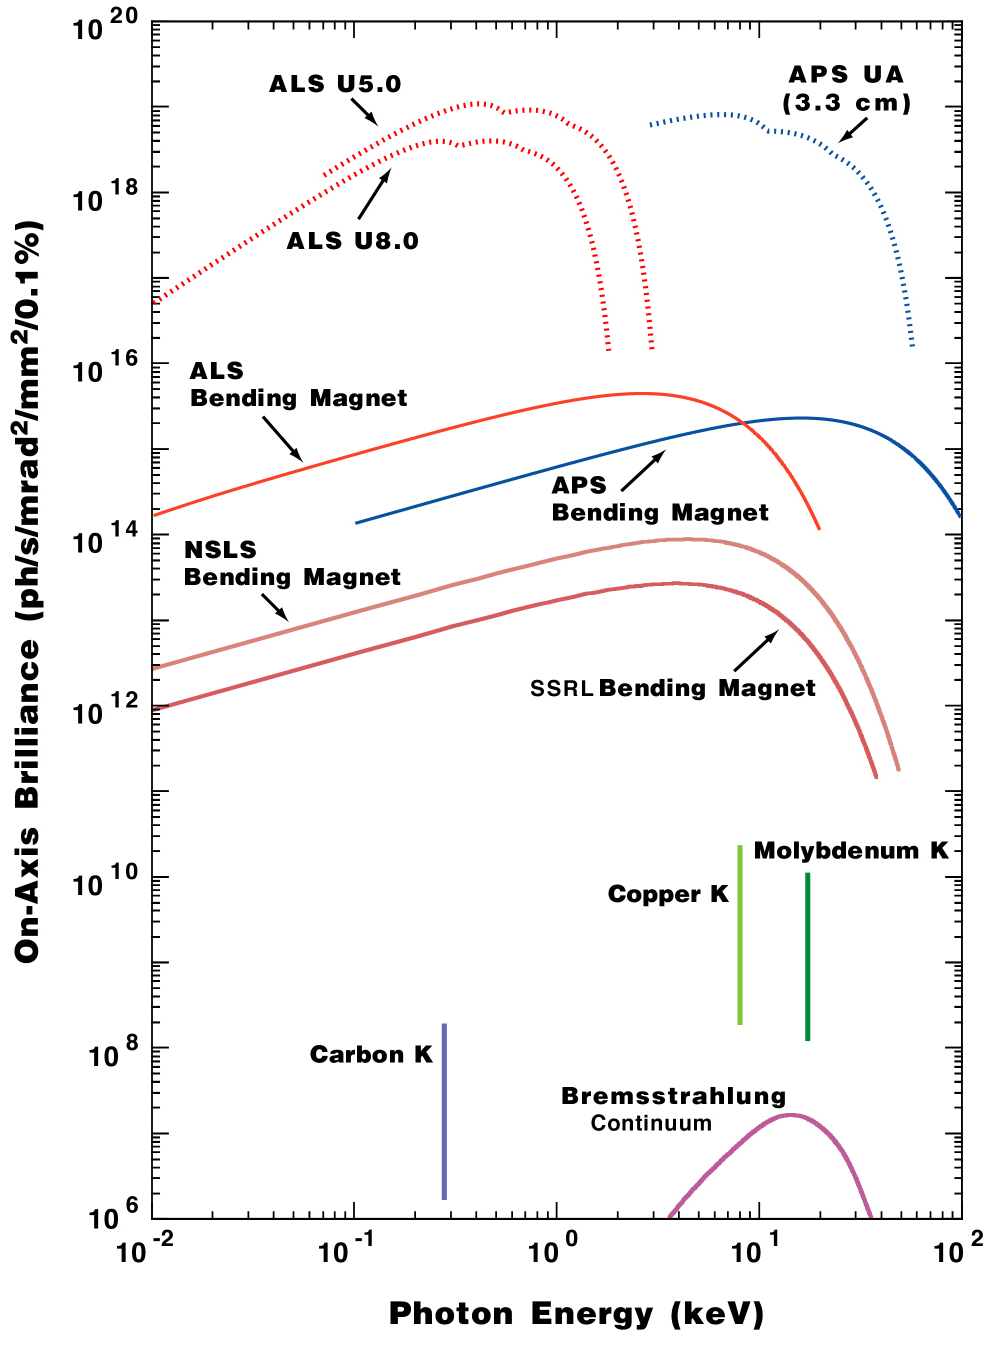
\includegraphics[width=57mm]{figs/misc/APS_und_spectra}
      }
    \end{column}
    \begin{column}{80mm}
    \onslide+<1->{

      {\RedEmph{Brilliance}}: flux of monochromatic X-rays in a highly
      collimated beam.

      \vmm
      Synchrotron beams are high flux {\bf{and}} highly collimated.
      
      }

      \onslide+<2->
      \vmm      \hrule       \vmm

      Modern synchrotrons are large ($\sim 1 \rm \, km$
      circumference), with dozens of beamlines

      \vmm
    \begin{center}      
      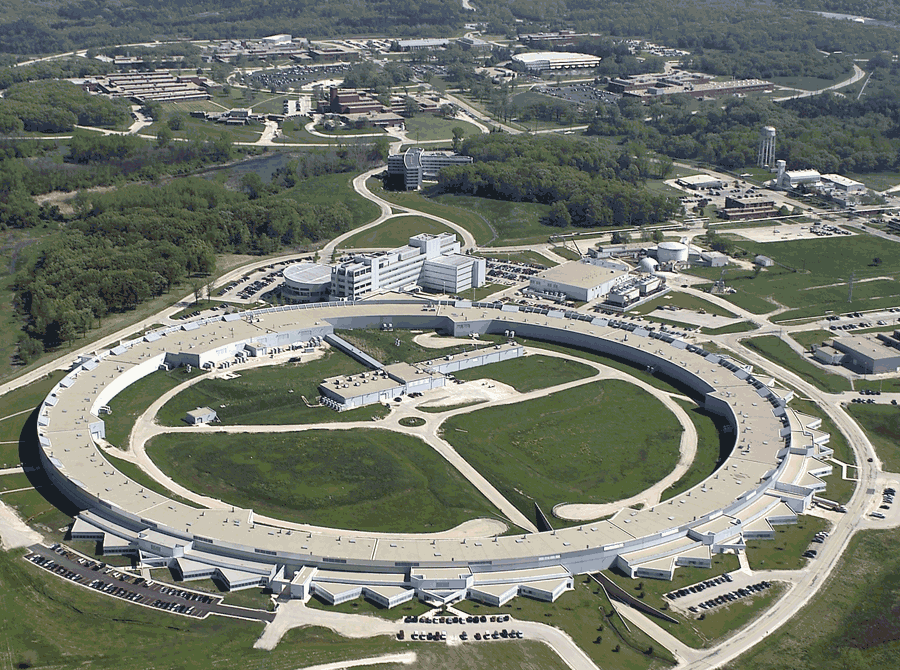
\includegraphics[width=52mm]{figs/misc/APS_aerial1}
    \end{center}

      Advanced Photon Source (APS) at Argonne National Lab: $\sim$ 60
      simultaneous, independent X-ray beamlines, each doing different
      science experiments.

    \end{column}
  \end{columns}

\end{slide}


\begin{slide}{Synchrotron: Beamlines }

 \vmm
\begin{columns}[T]
  \begin{column}{55mm}
    \onslide+<1->{

    \begin{center}
      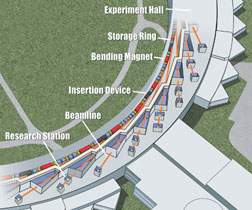
\includegraphics[width=45mm]{figs/misc/APS_aerial2}
    \end{center}

    The APS has 35 Sectors, each with:

    \begin{itemize}
        \item 1 Bending Magnet and 1 Undulator (high brightness)
          beamline.

        \item 200 days of beamtime per year.

        \item 25\% to 90\% of beamtime to peer-reviewed proposals.

        \end{itemize}
      }
      
    \end{column}
    \begin{column}{75mm}

      \onslide+<2->{
        \begin{center}
          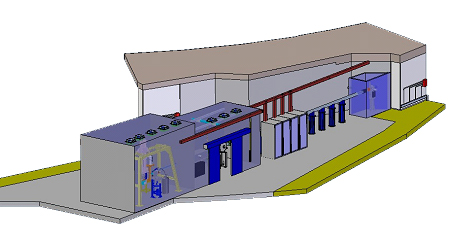
\includegraphics[width=53mm]{figs/misc/APS_beamline_layout}
        \end{center}
        

         \vmm {\RedEmph{A beamline}}: Pb enclosures (hutches) hold X-ray
         optics (monochromators, mirrors, slits) and experimental equipment,
         and protect people from radiation.

         \vmm Experiments happen at $\sim$ 40m from the X-ray source.

         \vmm Most beamlines dedicated to a technique or scientific discipline.

         \vmm Most beamlines run by ANL, some by outside groups.

       }
     \end{column}
   \end{columns}


\end{slide}


